
\documentclass[a4paper,11pt]{article}
\usepackage[a4paper, margin=8em]{geometry}

% usa i pacchetti per la scrittura in italiano
\usepackage[french,italian]{babel}
\usepackage[T1]{fontenc}
\usepackage[utf8]{inputenc}
\frenchspacing 

% usa i pacchetti per la formattazione matematica
\usepackage{amsmath, amssymb, amsthm, amsfonts}

% usa altri pacchetti
\usepackage{gensymb}
\usepackage{hyperref}
\usepackage{standalone}

% imposta il titolo
\title{Appunti Elettronica Digitale}
\author{Luca Seggiani}
\date{2026}

% imposta lo stile
% usa helvetica
\usepackage[scaled]{helvet}
% usa palatino
\usepackage{palatino}
% usa un font monospazio guardabile
\usepackage{lmodern}

\renewcommand{\rmdefault}{ppl}
\renewcommand{\sfdefault}{phv}
\renewcommand{\ttdefault}{lmtt}

% disponi il titolo
\makeatletter
\renewcommand{\maketitle} {
	\begin{center} 
		\begin{minipage}[t]{.8\textwidth}
			\textsf{\huge\bfseries \@title} 
		\end{minipage}%
		\begin{minipage}[t]{.2\textwidth}
			\raggedleft \vspace{-1.65em}
			\textsf{\small \@author} \vfill
			\textsf{\small \@date}
		\end{minipage}
		\par
	\end{center}

	\thispagestyle{empty}
	\pagestyle{fancy}
}
\makeatother

% disponi teoremi
\usepackage{tcolorbox}
\newtcolorbox[auto counter, number within=section]{theorem}[2][]{%
	colback=blue!10, 
	colframe=blue!40!black, 
	sharp corners=northwest,
	fonttitle=\sffamily\bfseries, 
	title=~\thetcbcounter: #2, 
	#1
}

% disponi definizioni
\newtcolorbox[auto counter, number within=section]{definition}[2][]{%
	colback=red!10,
	colframe=red!40!black,
	sharp corners=northwest,
	fonttitle=\sffamily\bfseries,
	title=~\thetcbcounter: #2,
	#1
}

% U.D.M
\newcommand{\amp}{\ensuremath{\mathrm{A}}}
\newcommand{\volt}{\ensuremath{\mathrm{V}}}
\newcommand{\meter}{\ensuremath{\mathrm{m}}}
\newcommand{\second}{\ensuremath{\mathrm{s}}}
\newcommand{\farad}{\ensuremath{\mathrm{F}}}
\newcommand{\henry}{\ensuremath{\mathrm{H}}}
\newcommand{\siemens}{\ensuremath{\mathrm{S}}}

% circuiti
\usepackage{circuitikz}
\usetikzlibrary{babel}

% disegni
\usepackage{pgfplots}
\pgfplotsset{width=10cm,compat=1.9}

% disponi codice
\usepackage{listings}
\usepackage[table]{xcolor}

\definecolor{codegreen}{rgb}{0,0.6,0}
\definecolor{codegray}{rgb}{0.5,0.5,0.5}
\definecolor{codepurple}{rgb}{0.58,0,0.82}
\definecolor{backcolour}{rgb}{0.95,0.95,0.92}

\lstdefinestyle{codestyle}{
		backgroundcolor=\color{black!5}, 
		commentstyle=\color{codegreen},
		keywordstyle=\bfseries\color{magenta},
		numberstyle=\sffamily\tiny\color{black!60},
		stringstyle=\color{green!50!black},
		basicstyle=\ttfamily\footnotesize,
		breakatwhitespace=false,         
		breaklines=true,                 
		captionpos=b,                    
		keepspaces=true,                 
		numbers=left,                    
		numbersep=5pt,                  
		showspaces=false,                
		showstringspaces=false,
		showtabs=false,                  
		tabsize=2
}

\lstdefinestyle{shellstyle}{
		backgroundcolor=\color{black!5}, 
		basicstyle=\ttfamily\footnotesize\color{black}, 
		commentstyle=\color{black}, 
		keywordstyle=\color{black},
		numberstyle=\color{black!5},
		stringstyle=\color{black}, 
		showspaces=false,
		showstringspaces=false, 
		showtabs=false, 
		tabsize=2, 
		numbers=none, 
		breaklines=true
}

\lstdefinelanguage{javascript}{
	keywords={typeof, new, true, false, catch, function, return, null, catch, switch, var, if, in, while, do, else, case, break},
	keywordstyle=\color{blue}\bfseries,
	ndkeywords={class, export, boolean, throw, implements, import, this},
	ndkeywordstyle=\color{darkgray}\bfseries,
	identifierstyle=\color{black},
	sensitive=false,
	comment=[l]{//},
	morecomment=[s]{/*}{*/},
	commentstyle=\color{purple}\ttfamily,
	stringstyle=\color{red}\ttfamily,
	morestring=[b]',
	morestring=[b]"
}

% disponi sezioni
\usepackage{titlesec}

\titleformat{\section}
	{\sffamily\Large\bfseries} 
	{\thesection}{1em}{} 
\titleformat{\subsection}
	{\sffamily\large\bfseries}   
	{\thesubsection}{1em}{} 
\titleformat{\subsubsection}
	{\sffamily\normalsize\bfseries} 
	{\thesubsubsection}{1em}{}

% disponi alberi
\usepackage{forest}

\forestset{
	rectstyle/.style={
		for tree={rectangle,draw,font=\large\sffamily}
	},
	roundstyle/.style={
		for tree={circle,draw,font=\large}
	}
}

% disponi algoritmi
\usepackage{algorithm}
\usepackage{algorithmic}
\makeatletter
\renewcommand{\ALG@name}{Algoritmo}
\makeatother

% disponi numeri di pagina
\usepackage{fancyhdr}
\fancyhf{} 
\fancyfoot[L]{\sffamily{\thepage}}

\makeatletter
\fancyhead[L]{\raisebox{1ex}[0pt][0pt]{\sffamily{\@title \ \@date}}} 
\fancyhead[R]{\raisebox{1ex}[0pt][0pt]{\sffamily{\@author}}}
\makeatother

\begin{document}
% sezione (data)
\section{Lezione del 24-03-26}

% stili pagina
\thispagestyle{empty}
\pagestyle{fancy}

% testo
Alla fine della scorsa lezione abbiamo visto un modello per il diodo ai \textit{piccoli segnali}, che consisteva nella linearizzazione attorno ad un punto di riposo $Q$. Questo corrispondeva effettivamente alla separazione del segnale studiato in una parte DC (data dal punto di linearizzazione $Q$), e una parte AC che studiavamo come piccolo segnale.

Vediamo quindi come sfruttare questo meccanismo per risolvere circuiti.

\subsubsection{Risoluzione di circuiti con diodi ai piccoli segnali}
Abbiamo quindi che un circuito con un diodo sottoposto ad un piccolo segnale può essere risolto prima considerando la parte DC del segnale secondo il classico modello ai grandi segnali (e.g. caduta costante), e quindi trattando lo specifico piccolo segnale. I due risultati si possono quindi combinare sfruttando il principo di sovrapposizione degli effetti. 

Il procedimento complessivo sarà:
\begin{enumerate}
\item Risolviamo prima il circuito nel punto di riposo con il modello del diodo per grandi segnali (e.g. grandi segnali) per trovare il comportamento al punto di riposo $Q$, o nello specifico la coppia $(V_Q, I_Q)$, di cui ricordiamo:
$$
V_{DQ} = Q, \quad I_{DQ} = I_S \left( e^{\frac{Q}{\eta V_T}} - 1\right)
$$
\item Quindi si potrà risolvere il circuito per il piccolo segnale usando il modello del diodo linearizzato, di cui ricordiamo:
$$
i_d = g_d v_d, \quad v_d = r_d i_d \quad \text{con} \quad
g_d = \frac{I_{DQ}}{\eta V_T}, \quad r_d = \frac{\eta V_T}{I_{DQ}}
$$
cioè il diodo viene trattato come una semplice resistenza $r_d$. Notiamo che $g_d$ (e ugualmente $r_d$) dipende dai parametri trovati sul punto di riposo, per cui bisogna prima fare l'analisi DC e solo dopo l'analisi AC.
\end{enumerate}

Chiaramente dovremo tenere a mente 2 cose:
\begin{enumerate}
	\item Prima di applicare questo processo si deve dividere il segnale agente sul circuito in una coppia DC, AC, cioè una componente costante (diciamo $V_{DC}$) e una componente che rappresenterà il piccolo segnale (diciamo $V_{AC}$). 

		Questo si farà \textit{spengendo} i segnali AC nell'analisi DC, e quindi usando un modello come la caduta costante, e ugualmente spengere i generatori DC nell'analisi AC, usando i parametri trovati dall'analisi AC per determinare i paremetri di risposta del circuito ai piccoli segnali.

	\item Applicando il principio di sovrapposizione degli effetti ad un circuito sostanzialmente non lineare, dovremmo commettere un errore. Questo è però giustificato dal fatto che se il segnale è piccolo, sostituiamo la curva esponenziale con la sua tangente nel punto $Q$. Una \textit{retta} in questo caso è un modello lineare abbastanza vicino al comportamento reale del componente.
\end{enumerate}

\subsection{Transistore bipolare}

Iniziamo a vedere il \textbf{transistore bipolare} (o \textbf{BJT}, \textit{Bipolar Junction Transistor}). Questo è un dispositivo a 2 porte, di cui però colleghiamo i negativi delle porte assieme, formando effettivamente un tripolo.

\begin{center}
\begin{circuitikz}

% Left port
\draw
(0.5,1.5) node[above] {$i_1$}
(0,1.5) node[left] {$+$}
(0,0.5) node[left] {$-$}
(0,1.5) to[short, o-] (1,1.5)
(0,0.5) to[short, o-] (1,0.5)
(0,1) node[left] {$v_1$};

% Right port
\draw
(6.5,1.5) node[above] {$i_2$}
(7,1.5) node[right] {$+$}
(7,0.5) node[right] {$-$}
(6,1.5) to[short, -o] (7,1.5)
(6,0.5) to[short, -o] (7,0.5)
(7,1) node[right] {$v_2$};

% Block
\draw[rounded corners, thick]
(1,2) rectangle (6,0);

\draw [dashed] (1, 0.5) -- (6, 0.5);

\end{circuitikz}
\end{center}

Idealmente viene rappresentato da un \textit{generatore di corrente controllato in corrente} (\textbf{GCCC}):

\begin{center}
\begin{circuitikz}

% Source side
\draw
(0,0) to[V=$v_S$] (0,3)
      to[R=$R_S$, i>^=$i_1$] (3.2,3)
      to[short] (3.2,0)
      -- (0,0);

\node at (2.5,0.25) {$-$};
\node at (2.5,1.5) {$v_1$};
\node at (2.5,2.75) {$+$};

% Controlled current source
\draw
(4.5,3) to[cisource, i=$A_i i_1$] (4.5,0)
	-- (3,0);

% Load
\draw
(4.5,0) -- (7,0)
      to[R, l_=$R_L$, i=$i_2$] (7,3)
      -- (4.5,3);

\node at (6,0.25) {$-$};
\node at (6,1.5) {$v_2$};
\node at (6,2.75) {$+$};

\draw[rounded corners, thick, dashed]
(3,3.2) rectangle (5.5, -0.2);

\end{circuitikz}
\end{center}

Nel circuito abbiamo rappresentato:
\begin{itemize}
	\item A sinistra una \textit{sorgente esterna}, cioè $v_S$, con la sua resistenza associata $R_S$;
	\item A destra una \textit{resistenza di carico}, che indichiamo come $R_L$.
\end{itemize}

Di base, un transistore bipolare sarà quindi un circuito che accetta una corrente a sinistra, e impone una corrente pari a questa ma modulata di un certo guadagno $A_i$ (che vedremo subito) a destra (nell'esempio specifico, accetta una corrente imposta dal generatore $v_S$ e fa passare una corrente sul carico $R_L$).

\par\smallskip

\noindent
\textbf{\textsf{Considerazioni sui guadagni}}

\noindent
Vediamo nel dettaglio cosa rappresenta il parametro $A_i$.
Di un transistore possiamo calcolare il \textit{guadagno di corrente} complessivo $A_i$ come:
$$
i_2 = A_i i_1 \implies A_i = \frac{i_2}{i_S} = \frac{i_2}{i_1}
$$
visto che la corrente sul generatore $v_S$ è $i_1$.

Nel suo uso generico, come abbiamo visto, si accoppia un transistor con una rete esterna che comprende un generatore di segnale di bassa potenza e un carico.
L'accoppiamento con la rete esterna (in particolare l'esistenza delle resistenze $R_S$ alla sorgente e $R_L$ al carico) permette di definire un \textit{guadagno di tensione} complessivo $A_v$:
$$
v_2 = -R_L i_2 = -R_L A_i i_1 = -R_L A_i \frac{v_s}{R_S}
$$
per cui possiamo dire, analogamente al guadagno di corrente complessivo $A_i$:
$$
A_v = \frac{v_2}{v_s} = -\frac{R_L A_i \frac{v_S}{R_S}}{ v_s } = -\frac{R_L}{R_S} A_i 
$$

Chiamiamo questi guadagni anche \textit{attenuazioni} o \textit{amplificazioni} sulla base dei loro valori:
$$
A_i = \frac{i_\mathrm{out}}{i_\mathrm{in}} \quad \text{(guadagno di corrente)} \quad
\begin{cases}
	A_i > 1 \quad \text{(amplificazione di corrente)} \\
	A_i < 1 \quad \text{(attenuazione di corrente)}
\end{cases}
$$

$$
A_v = \frac{v_\mathrm{out}}{v_\mathrm{in}} \quad \text{(guadagno di tensione)} \quad
\begin{cases}
	A_v > 1 \quad \text{(amplificazione di tensione)} \\
	A_v < 1 \quad \text{(attenuazione di tensione)}
\end{cases}
$$

\par\smallskip

\noindent
\textbf{\textsf{Considerazioni di potenza}}

\noindent
Parliamo quindi della potenza erogata da un lato e dall'altro del transistore. Abbiamo che:
\begin{itemize}
\item Sul \textit{carico} $R_L$, eroghiamo la potenza:
$$
P_L = -v_2 i_2
$$
\item La \textit{sorgente}, di per sé, eroga la potenza:
$$
P_S = v_s i_1
$$
\end{itemize}

Possiamo quindi definire un guadagno complessivo anche sulle \textit{potenze} $A_P$, che sarà uguale a:
$$
A_P = \frac{P_L}{P_S} = -\frac{v_2 i_2}{v_s i_1} = -A_i A_v = A_i^2 \frac{R_L}{R_S} = - A_v^2 \frac{R_S}{R_L}
$$

Notiamo quindi una prima particolarità dei transistor: i componenti \textit{attivi} (come i \textbf{BJT} o i \textbf{MOSFET}, \textit{Metal–Oxide–Semiconductor Field-Effect Transistor}) permettono di ottenere valori di $A_P > 1$, cioè ricavare più potenza al carico di quanta ne viene erogata dalla sorgente (chiaramente sotto alimentazione esterna).

Questo è il primo caso di utilizzo del transistor, cioè come \textit{amplificatore} di potenza.

\subsubsection{Modello fisico del transistor}
Finora abbiamo trattato il transistor come un componente idealizzato, che si comportava come un \textit{GCCC}, e abbiamo quindi calcolato i valori di guadagno in \textit{corrente}, \textit{tensione} e \textit{potenza}.

Adesso vediamo come, dal punto di vista fisico, si realizza un transistore a giunzione bipolare. Innanzitutto, \textit{bipolare} significa due giunzioni PN poste una di seguito all'altra e orientate in senso inverso.

Per qeusto motivo esistono 2 tipi principali di transistore bipolare: il transistore \textbf{PNP} (che lega una giunzione PN ad una giunzione NP) e il transistore \textbf{NPN} (che lega una giunzione NP ad una giunzione PN):
\begin{itemize}
	\item \textbf{\textsf{Transistore PNP}} \\
Viene formato da una giunzione PN e una giunzione NP:
\begin{center}
	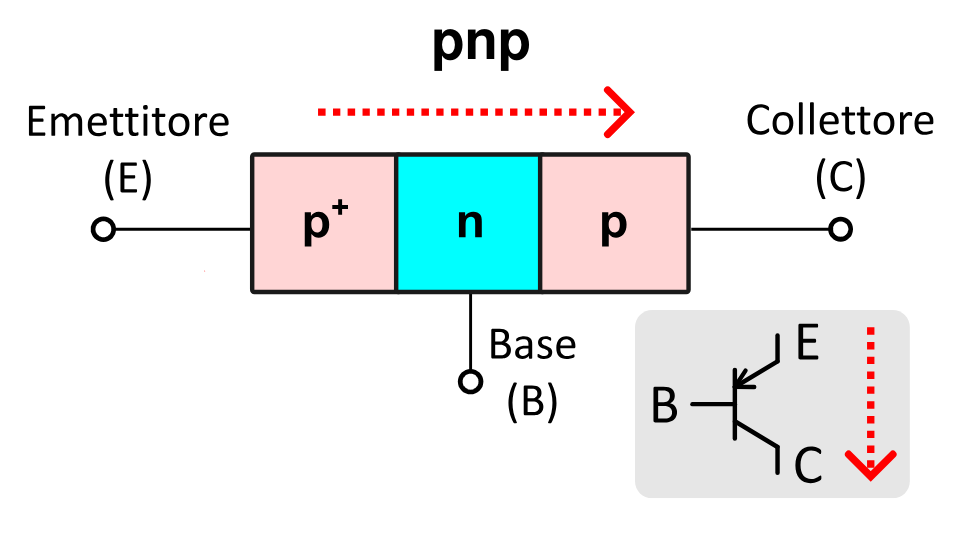
\includegraphics[scale=0.28]{../figures/pnp.png}
\end{center}
Nel transistore PNP abbiamo quindi una regione $\text{P}^+$ fortemente drogata (da cui il $+$ ad apice), una regione N leggermente drogata, e una regione P meno drogata della prima regione $\text{P}^+$.

I poli connessi a sinistra e destra sono detti \textit{emettitore} (\textbf{E}) e \textit{collettore} (\textbf{C}). La regione N è ancorata alla \textit{base} \textbf{B}. Il grafico in basso a destra mostra la direzione della corrente tipica (da emettitore a collettore) del transistore PNP;
	
	\item \textbf{\textsf{Transistore NPN}} \\
Viene formato da una giunzione NP e una giunzione PN:
\begin{center}
	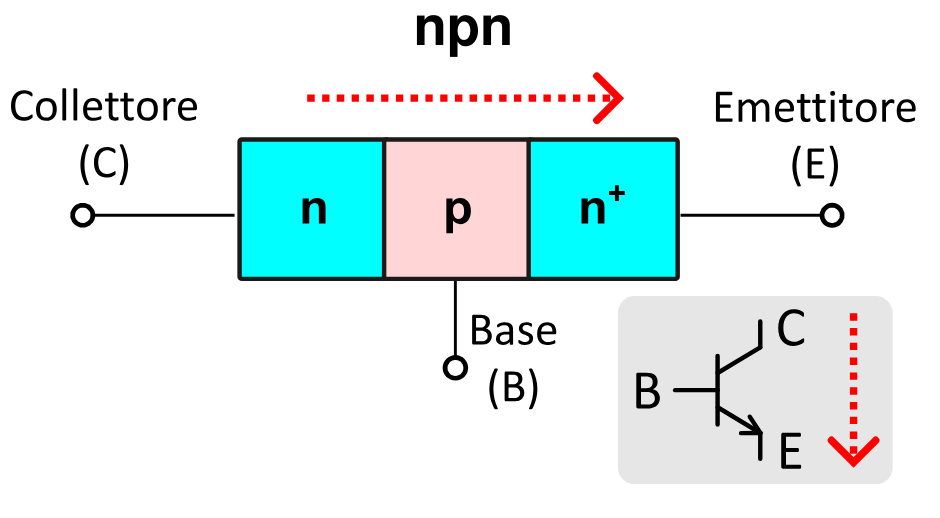
\includegraphics[scale=0.28]{../figures/npn.png}
\end{center}
Nel transistore NPN abbiamo quindi una regione $\text{N}$, una regione P leggermente drogata, e una regione $\text{N}^+$ più drogata della prima regione N.

I poli connessi a sinistra e destra sono stavolta \textit{collettore} (\textbf{C}) ed \textit{emettitore} (\textbf{E}). Stavolta la regione P è ancorata alla \textit{base} \textbf{B}. Il grafico in basso a destra mostra la direzione della corrente tipica (da collettore ad emettitore) del transistore NPN;
\end{itemize}

Riguardo ai poli che abbiamo nominato, vale che in genere:
\begin{itemize}
	\item L'\textit{emettitore} (\textbf{E}) si occupa di \textit{emettere} i portatori di carica;
	\item Il \textit{collettore} (\textbf{C}) si occupa di \textit{raccogliere} i portatori di carica;
	\item La \textit{base} (\textbf{B}) si occupa di \textit{modulare} il passaggio dei portatori di carica fra le zone emettitore e collettore.
\end{itemize}

Il risultato è che in un transistore PNP una corrente passa fra collettore ed emettitore quando si applica una piccola corrente \textit{negativa} alla base, mentre in un transistore NPN una corrente passa fra emettitore e collettore quando si applica una piccola corrente \textit{positiva} alla base.

\par\smallskip

\noindent
\textbf{\textsf{Trattazione nel caso PNP}}

\noindent
Continuiamo la trattazione fisica nel dettaglio, prendendo a riferimento il transistore \textit{PNP} (la descrizione del NPN sarà pressapoco analoga). Consideriamo quindi un modello semplificato che prende le due giunzioni (PN ed NP) separatamente. Inoltre, assumiamo che fra base ed emettitore sia imposto un voltaggio positivo (polarizzazione positiva della regione PN), e che fra base e collettore sia imposto un voltaggio negativo (polarizzazione negativa della regione NP).

\begin{itemize}
	\item \textbf{\textsf{Giunzione PN}} \\
A sinistra il transistore PNP si presenta come segue:
\begin{center}
	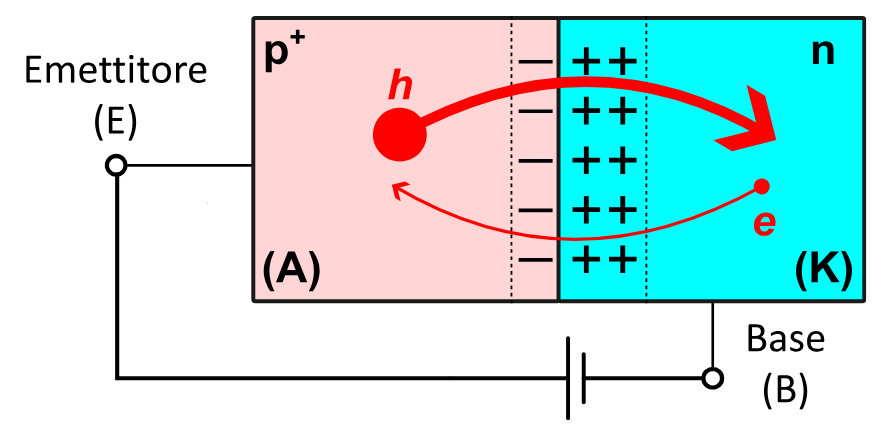
\includegraphics[scale=0.22]{../figures/pn.png}
\end{center}
Abbiamo quindi la giunzione PN che viene messa in polarizzazione \textit{diretta} dal voltaggio applicato fra emettitore e base.

Questa è esattamente la situazione che abbiamo studiato in 5.1, e porta questa parte del transistore a comportarsi come un diodo in conduzione: applicando voltaggio in polarizzazione diretta i conduttori maggioritari della zona P (le lacune) si spostano nella regione N, la barriera di potenziale si abbassa, e si ha quindi conduzione di corrente da E a B (con crescita esponenziale all'aumentare del voltaggio applicato).

Inoltre, nel PNP si ha che la zona $\text{P}^+$ è molto drogata, cioè:
$$
N_A >> N_D
$$
e quindi il flusso di $h$ è molto maggiore del flusso di $e$.
L'effetto complessivo di questa situazione sarà quindi che un grande numero di lacune $h$ verranno spinte (a volte si dice \textit{iniettate}) nella regione N centrale. 

	\item \textbf{\textsf{Giunzione NP}} \\
A destra il transistore PNP si presenta come segue:
\begin{center}
	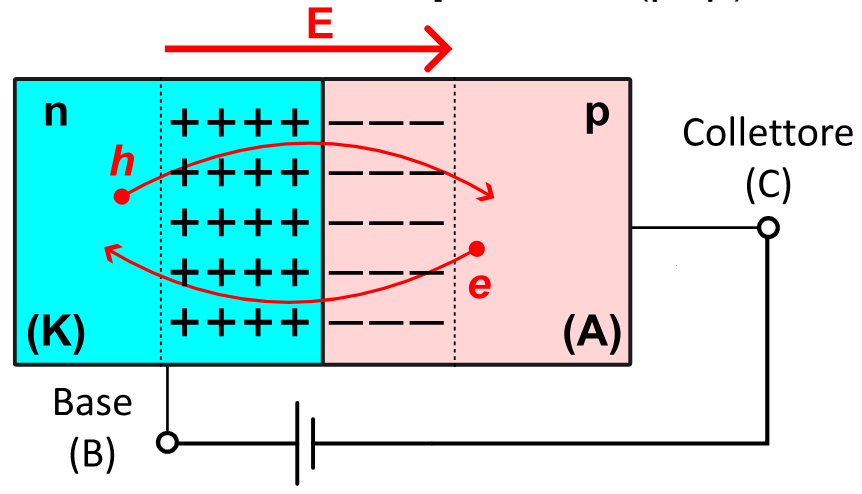
\includegraphics[scale=0.22]{../figures/np.png}
\end{center}
In questo caso abbiamo sempre una giunzione PN, stavolta in polarizzazione inversa fra collettore e base.

% SEI ARRIVATO QUI COGLIONE !!!

% Visto che siamo in conduzione inversa (sempre da 5.1), la barriera di potenziale si alzerà, la zona di svuotamento si allargherà, e si avrà una corrente data dai portatori minoritari, ovvero le lacune (limitata dalla generazione termica ed indipendente dal campo $E$).

\end{itemize}

Nel complesso, quindi, il transistore PNP si mostra come segue:
\begin{center}
	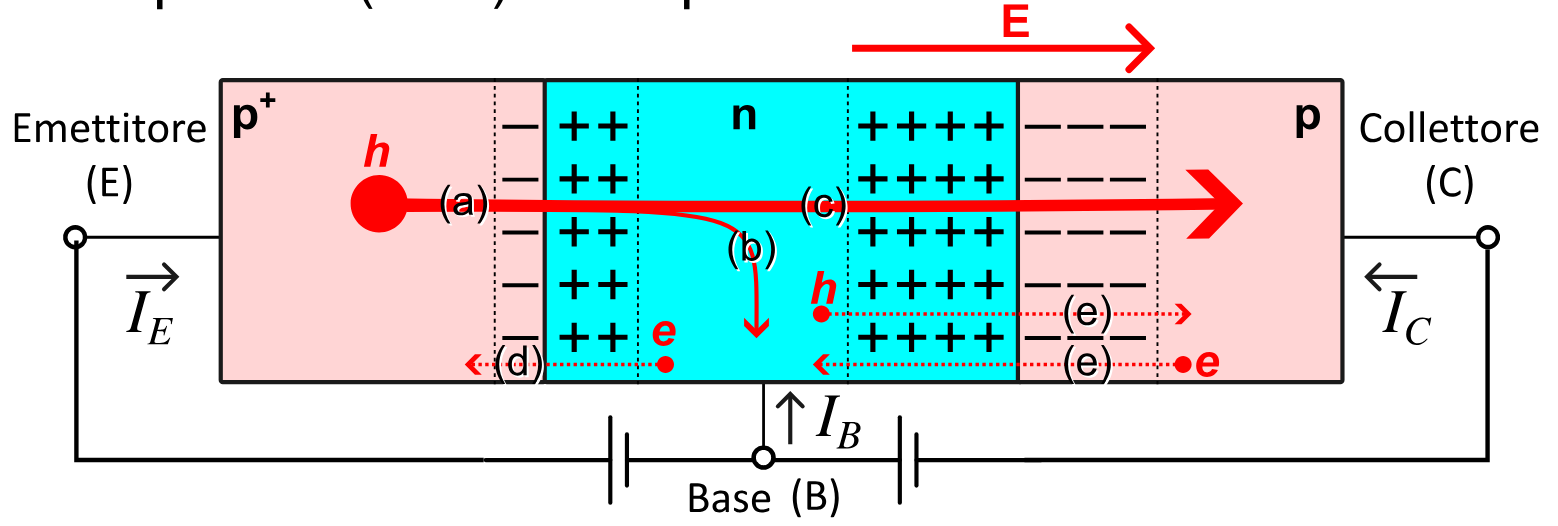
\includegraphics[scale=0.22]{../figures/full_pnp.png}
\end{center}

In \textit{Zona Attiva Direttta} (\textit{ZAD}), quindi, si ha la giunzione BE (cioè la giunzione PN collegata ad emettitore e base) in polarizzazione diretta, e la giunzione BC (cioè la giunzione NP collegata a base e collettore) in polarizzazione inversa. In simboli:
$$
V_{EB} > 0, \quad V_{CB} < 0
$$

Questo significherà:
\begin{enumerate}
	\item Grande flusso di lacune $h$ da E e B dato dalla corrente di diffusione (cioè dalla giunzione PN in polarizzazione diretta);
	\item Una piccola porzione di $h$ che si ricombinano in base, la cui zona nuetra ha un’alta concentrazione di $e$ (in quanto il campo $E$ applicato riporta gli $n$ all'interno della zona N);
	\item La parte rimanente degli $h$ arriva alla zona di svuotamento BC dove è presente un forte campo elettrico: queste sono le cariche che riforniscono la giunzione BC in inversa.
\end{enumerate}

# finisci

\subsubsection{Modello di Ebers-Moll}
Il modello di \textit{Ebers-Moll} per il transistore bipolare permette di descrivere questo componente ai grandi segnali. Il modello si deriva direttamente dalla rappresentazione fisica del transistore.

\begin{center}
	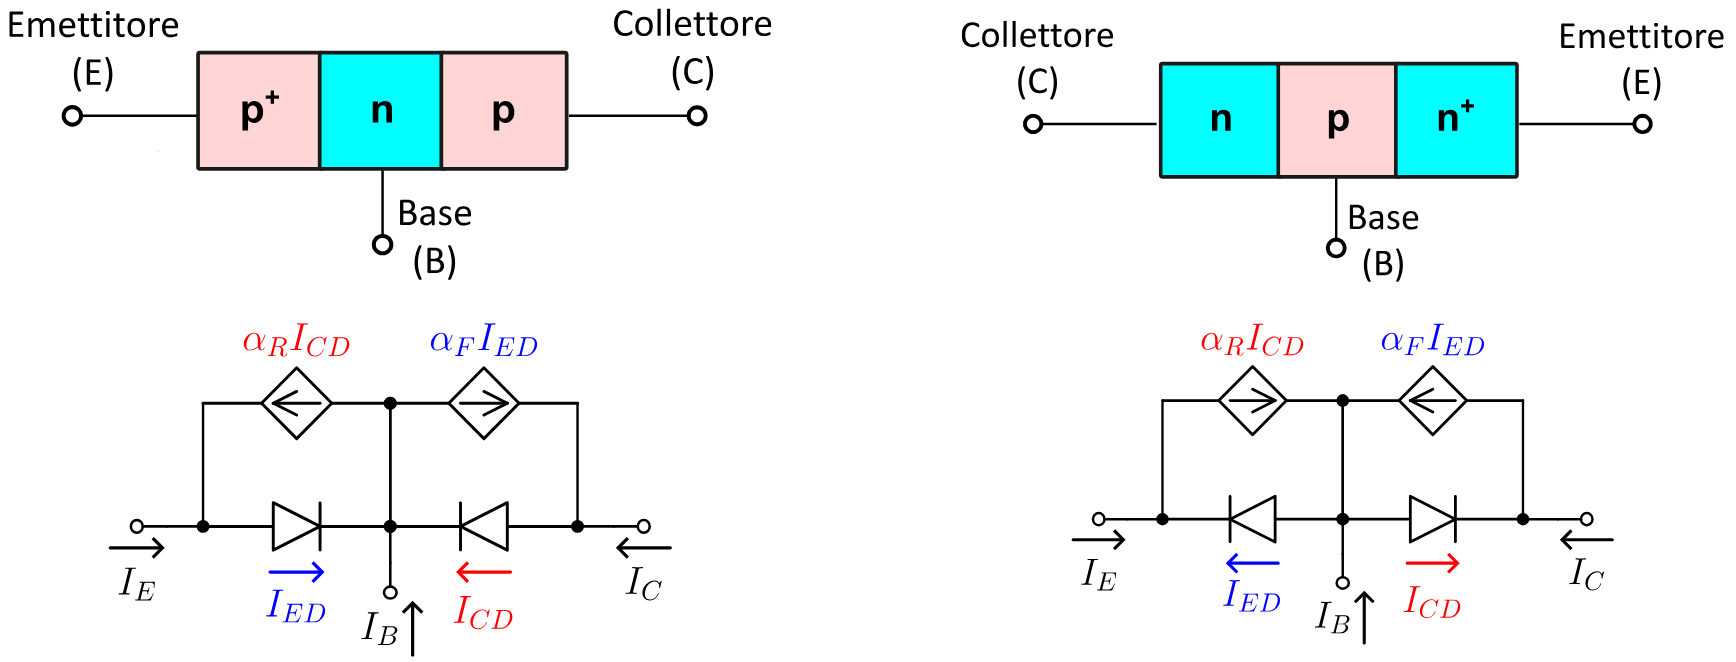
\includegraphics[scale=0.24]{../figures/ebers.png}
\end{center}

Modellizziamo quindi il transistor come una coppia di diodi che pilotano generatori di corrente. Questi sono:
\begin{itemize}
	\item Rivolti da E a B e da E a C nel caso del transistore PNP;
	\item Rivolti da B ad E e da B a C nel caso del transistore NPN.
\end{itemize}

I generatori di correnti chiudono le maglie seguendo le direzioni dei diodi. Le costanti di proporzionalità sono 2, cioè $\alpha_F$ e $\alpha_R$:
\begin{itemize}
	\item $\alpha_F$ è la frazione di corrente \textit{diretta}, con:
$$
0.98 < \alpha_F < 0.998
$$
	\item $\alpha_R$ è la frazione di corrente \textit{inversa}, con:
$$
0.4 < \alpha_R < 0.8
$$
\end{itemize}
Fra queste costanti, a causa del diverso drogaggio delle regioni P (nel PNP) o N (nel NPN), saranno diverse fra di loro, e in particolare varrà:
$$
\alpha_F I_{ES} = \alpha_R I_{CS}
$$
Dove $I_{ES}$ e $I_{CS}$ sono le correnti di saturazione dei diodi sull'emettitore e sul collettore.

Prendiamo l'esempio specifico del transistore PNP.
Possiamo discutere questo modello introducendo l'equazione di Shockley per i diodi:
$$
\begin{cases}
	I_{ED} = I_{ES} \left( e^\frac{V_{EB}}{V_T} - 1 \right) \\
	I_{CD} = I_{CS} \left( e^\frac{V_{CB}}{V_T} - 1 \right) \\
\end{cases}
$$
e quindi scrivendo le equazioni nodali:
$$
\begin{cases}
I_E = I_{ED} - \alpha_R I_{CD} \\
I_C = I_{CD} - \alpha_F I_{ED} \\
I_B = -I_E - I_C
\end{cases}
$$
che sostituendo ci dà:
$$
\begin{cases}
I_E = I_{ES} \left( e^\frac{V_{EB}}{V_T} - 1 \right) - \alpha_R I_{CS} \left( e^\frac{V_{CB}}{V_T} - 1 \right) \\
I_C = I_{CS} \left( e^\frac{V_{CB}}{V_T} - 1 \right) - \alpha_F I_{ES} \left( e^\frac{V_{EB}}{V_T} - 1 \right)
\end{cases}
$$

% trova per npn

Sempre nel PNP, in \textit{zona attiva diretta}, abbiamo:
$$
V_{EB} >> V_T, \quad V_{CB} << 0
$$
cioè regione PN in polarizzazione diretta e regione NP in polarizzazione inversa, per cui possiamo approssimare gli esponenziali:
$$
\begin{cases}
	I_E = I_{ES} e^{\frac{V_{EB}}{V_T}} - \alpha_R I_{CS} (-1) \\
	I_C = I_{CS} (-1) - \alpha_F I_{ES} e^{\frac{V_{EB}}{V_T}}
\end{cases}
\implies
\begin{cases}
	I_E = I_{ES} e^{\frac{V_{EB}}{V_T}} + \alpha_R I_{CS} \\
	I_C = -I_{CS} - \alpha_F I_{ES} e^{\frac{V_{EB}}{V_T}}
\end{cases}
$$
e semplificando ancora (gli esponenziali vincono sui termini lineari):
$$
\begin{cases}
	I_E = I_{ES} e^{\frac{V_{EB}}{V_T}} \\
	I_C = \alpha_F I_{ES} e^{\frac{V_{EB}}{V_T}}
\end{cases}
$$
Mettendo a comune la $I_E$:
$$
I_E = I_{ES} e^{\frac{V_{EB}}{V_T}}
$$
si ottiene:
$$
\begin{cases}
I_C = - \alpha_F I_E \\
I_B = -(I_E + I_C) = - (1 - \alpha_F) I_E
\end{cases}
$$

Ci siamo quindi riportati al modello a \textit{generatore di corrente pilotato in corrente}, dove abbiamo il fattore di proporzionalità fra la corrente applicata alla base e quella misurata al collettore:
$$
\beta_F = \frac{I_C}{I_B} = \frac{\alpha_F}{1 - \alpha_F}, \quad I_C = \beta_F I_B
$$

\end{document}
